\section{IGSN in the Field}

\begin{sectionframe} % Custom environment required for section slides
	\frametitle{IGSN in the Field}
	\framesubtitle{Deploying persistent sample identifiers}

    \vfill
    
FAIMS Project interest in IGSNs began when CSIRO required their assignment to samples during fieldwork using FAIMS Mobile.

% 	This is on another line
\end{sectionframe}

%----------------------------------------------------------------------------------------

\begin{frame}{CSIRO fieldwork}
 \begin{figure}[SF]
    \centering
    \vspace{-0.5cm}
        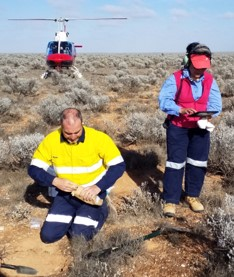
\includegraphics[height=.70\textheight]{figures/CSIRO-fieldwork.jpg}
        \caption{Geological sampling fieldwork in remote Western Australia}
        \label{fig:CSIRO geological sampling fieldwork}
 \end{figure}
\end{frame}


%----------------------------------------------------------------------------------------

\begin{frame}{Why FAIMS and IGSN?}
    \begin{itemize}
        \item Dedicated sample PIDs.
        \item Separates registration of identifier and description of object.
        \item Useful during fieldwork across various domains.
        \item Can be assigned to different materials.
        \item Description defined by particular disciplinary community.
        \item IGSN aligns with FAIMS philosophy: designed specifically to address challenges encountered during fieldwork, but adaptable across many disciplines and projects.
    \end{itemize}
\end{frame}
%----------------------------------------------------------------------------------------

\begin{frame}{CSIRO fieldwork approach}
    \begin{itemize}
        \item Considered several approaches, including on-demand printing of IGSNs in the field using a portable Bluetooth label printer.
        \item Pre-printing of labels proved most reliable and efficient.
        \item Potential IGSNs could be generated ahead of time, using rules making them globally unique.
        \item Since IGSN URLs follow a known pattern, URLs could be encoded.
        \item Printed as 'raffle-book' labels (two copies, one for sample, one for record) with human-readable text and a QR code.
        \item Assigned to sample and tied to record by scanning QR code in the FAIMS Mobile application when the sample was taken in field.
        \item After fieldwork, used IGSNs registered.
    \end{itemize}
\end{frame}


%----------------------------------------------------------------------------------------

\begin{frame}{CSIRO IGSN label}
 \begin{figure}[SI]
    \centering
    \vspace{-0.5cm}
        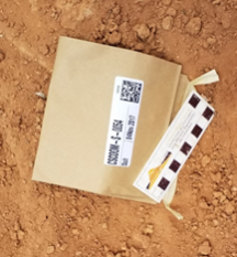
\includegraphics[height=.70\textheight]{figures/CSIRO-IGSN.png}
        \caption{Label including QR code containing IGSN number and URL}
        \label{fig:CSIRO IGSN label}
 \end{figure}
\end{frame}

% %----------------------------------------------------------------------------------------

\begin{frame}{Planned application in archaeology}
    \begin{itemize}
        \item Delayed due to COVID-related interruptions to fieldwork.
        \item Planned use at the Australian Research Council funded project ‘History, heritage and environmental change in a deindustrialised landscape’ (LP190100900).
        \item Historical archaeology fieldwork including surface survey and targeted excavations across an extensive landscape of late-19th / early-20th century mining settlements.
        \item Uses include environmental samples and artefacts.
        \item Will adopt the CSIRO approach (pre-printed labels).
        \item Flexibility across domains and ability to register PID post facto are the keys to usability.
    \end{itemize}
\end{frame}

%----------------------------------------------------------------------------------------

\begin{frame}{Blue Mountains fieldwork}
 \begin{figure}[BM]
    \centering
    \vspace{-0.5cm}
        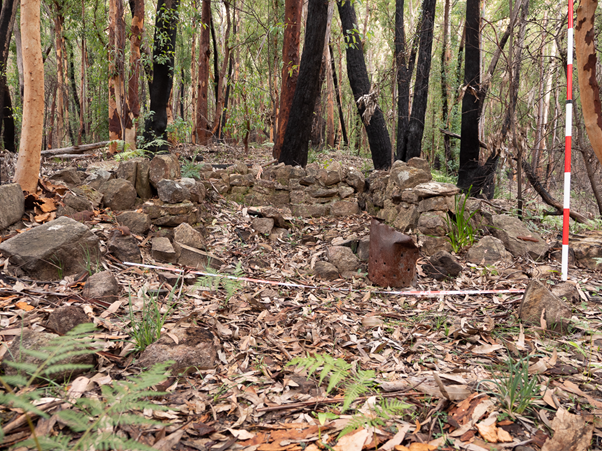
\includegraphics[height=.70\textheight]{figures/BM-fieldwork.png}
        \caption{Typical mining settlement remains and environs}
        \label{fig:Blue Mountains historical archaeology fieldwork}
 \end{figure}
\end{frame}
%----------------------------------------------------------------------------------------
\begin{frame}{Outcomes of IGSN use}
    \begin{itemize}
        \item Ability to track samples, sub-samples.
        \item Ability to cite samples.
        \item Ability to cross-link with DOI and ORCiD (especially in light of the DataCite partnership).
        \item Anyone encountering an unknown bag or object in future can scan or type in code to identify sample - eliminates (too frequent) inquiries about 'what is this sample / artefact and where did it come from'?
    \end{itemize}
\end{frame}
%----------------------------------------------------------------------------------------